\subsection{Matrix-Chain of Size n = 6:}

The first test consist in calculate the optimal parenthesization for the matrices in Table 2, The output of our program it's captured in Figure 4.1.0. \hfill \break

\begin{center}
\begin{tabular}{c c c c c c c}
\toprule
\toprule
\hspace{5px} Matrix \hspace{5px} & \hspace{20px} $A_{1}$ \hspace{20px} & \hspace{20px} $A_{2}$ \hspace{20px} & \hspace{20px} $A_{3}$ \hspace{20px} & \hspace{20px} $A_{4}$ \hspace{20px} & \hspace{20px} $A_{5}$ \hspace{20px} & \hspace{20px} $A_{6}$ \hspace{20px} \\
\toprule
\toprule
Dimensions & 30 x 35 & 35 x 15 & 15 x 5 & 5 x 10 & 10 x 20 & 20 x 25 \\
\bottomrule
\end{tabular}
\linebreak \linebreak Table 2: Matrix-chain of n = 6.
\end{center} \hfill

\begin{figure}[H]
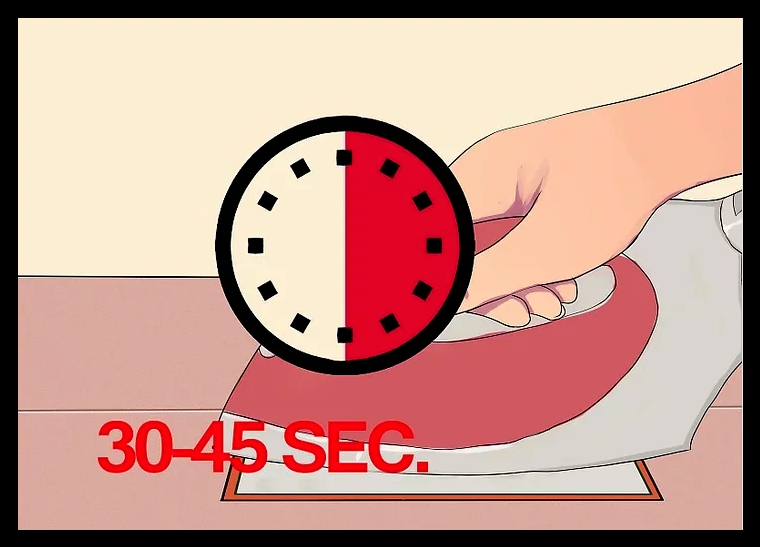
\includegraphics[height = 8cm, width = 16.5cm]{2.png}
\centering \linebreak \linebreak {\itshape\small Figure 4.1.0: Console output for Table 2 matrices.}
\end{figure} \hfill

As we can see in Figure 4.1.0 we have 2 tables; {\itshape m} and {\itshape s}. As we have explained in section 3, the table {\itshape s} are the pivots for the optimal parenthesization and table {\itshape m} it's the one that contains the minimum cost. This minimum cost it's stored in row 2, column 7 which is {\itshape 15, 125}. Finally in the bottom we can visualize the correct parenthesization. 

\pagebreak

Also for this test, we don't capture the others parenthesizations as in Figure 4.1.0, but we captured all the costs for all configurations as we can see in Figure 4.1.1, and also we corroborate that the configuration in Figure 4.1.0 it's the optimal. \hfill \break

\begin{multicols}{3}
\begin{figure}[H]
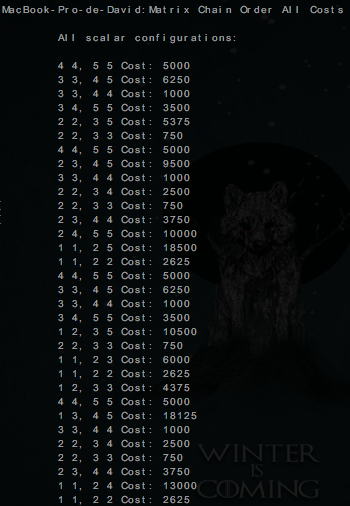
\includegraphics[height = 8cm, width = 6cm]{t1-1.png}
\centering \linebreak \linebreak
\end{figure} \hfill \break

\begin{figure}[H]
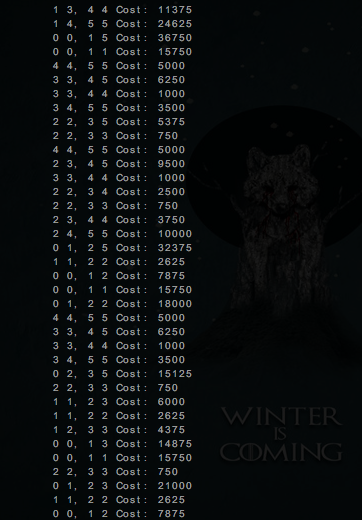
\includegraphics[height = 8cm, width = 6cm]{t1-2.png}
\centering \linebreak \linebreak {\itshape\small Figure 4.1.1: All configurations output.}
\end{figure} \hfill \break

\begin{figure}[H]
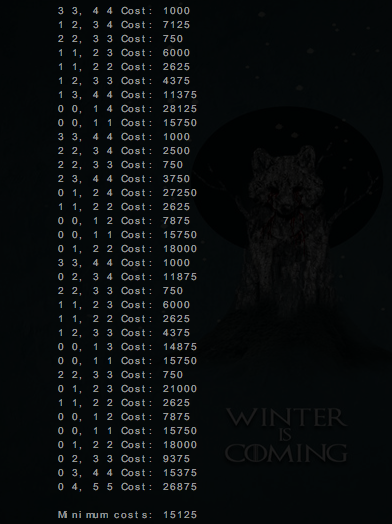
\includegraphics[height = 8cm, width = 6cm]{t1-3.png}
\centering \linebreak \linebreak
\end{figure} \hfill \break
\end{multicols}

\pagebreak